% Contribua em https://github.com/gabriel-del/latex-abnt-template
\documentclass[
	% -- opções da classe memoir --
	12pt,				% tamanho da fonte
	openright,			% capítulos começam em pág ímpar (insere página vazia caso preciso)
	oneside,			% Para impressão simples. Para impressão frente e verso, use twoside
	a4paper,			% tamanho do papel.
	% -- opções do pacote babel --
	english,			% idioma adicional para hifenização
	brazil				% o último idioma é o principal do documento
	]{abntex2}
\usepackage{lmodern}			% Usa a fonte Latin Modern
\usepackage[T1]{fontenc}		% Selecao de codigos de fonte.
\usepackage[utf8]{inputenc}		% Codificacao do documento (conversão automática dos acentos)
\usepackage{lastpage}			% Usado pela Ficha catalográfica
\usepackage{indentfirst}		% Indenta o primeiro parágrafo de cada seção.
\usepackage{color}				% Controle das cores
\usepackage{graphicx}			% Inclusão de gráficos
\usepackage{microtype} 			% para melhorias de justificação
\usepackage{listings}
\usepackage{tikz}
\usepackage{float}
\usepackage[brazilian,hyperpageref]{backref}
% Escolha um dos formatos de citação:
% Citação estilo IEEE: "Lorem ipsum [1]."
\usepackage[alf]{abntex2cite}
% \citebrackets[]
% Citação estilo "Lorem ipsum (Autor, 1986)."
% \usepackage[alf]{abntex2cite}	% Citações padrão ABNT
\usepackage{listings}
\definecolor{codegreen}{rgb}{0,0.6,0}
\definecolor{codegray}{rgb}{0.5,0.5,0.5}
\definecolor{codepurple}{rgb}{0.58,0,0.82}
\definecolor{backcolour}{rgb}{0.95,0.95,0.92}
\lstdefinestyle{mystyle}{
  extendedchars=false
  escapeinside="
  backgroundcolor=\color{backcolour},   commentstyle=\color{codegreen},
  keywordstyle=\color{magenta},
  numberstyle=\tiny\color{codegray},
  stringstyle=\color{codepurple},
  basicstyle=\ttfamily\footnotesize,
  breakatwhitespace=false,
  breaklines=true,
  captionpos=b,
  keepspaces=true,
  numbers=left,
  numbersep=5pt,
  showspaces=false,
  showstringspaces=false,
  showtabs=false,
  tabsize=2,
  numberbychapter=false
}
\lstset{style=mystyle}
\renewcommand{\lstlistingname}{Código}
\graphicspath{ {./pictures/} }
\renewcommand{\backrefpagesname}{Citado na(s) página(s):~}
\renewcommand{\backref}{}
\renewcommand*{\backrefalt}[4]{
	\ifcase #1 Nenhuma citação no texto.
	\or Citado na página #2.
	\else Citado #1 vezes nas páginas #2.
	\fi}
\titulo{Template Latex ABNT2}
\autor{Gabriel Del Cesare Barros}
\local{Recife}
\data{2020}
\orientador{ORIENTADOR}
\coorientador{} % Deixar vazio caso não haja
\instituicao{
  UNIVERSIDADE FEDERAL DE PERNAMBUCO
  \par
  CENTRO
  \par
  DEPARTAMENTO}
\tipotrabalho{Trabalho de Conclusão de Curso de Graduação}
\preambulo{}
\definecolor{blue}{RGB}{41,5,195}
\makeatletter
\hypersetup{
    pagebackref=true,
		pdftitle={\@title},
		pdfauthor={\@author},
    	pdfsubject={\imprimirpreambulo},
	    pdfcreator={LaTeX with abnTeX2},
		pdfkeywords={abnt}{latex}{abntex}{abntex2}{trabalho acadêmico},
		colorlinks=true,       % false: boxed links; true: colored links
    	linkcolor=black,     % color of internal links
    	citecolor=blue,      % color of links to bibliography
    	filecolor=magenta,   % color of file links
		urlcolor=blue,
		bookmarksdepth=4
}
% \def\UrlLeft{} \def\UrlRight{} %Contorno dos <links>
\makeatother
\setlength{\parindent}{1.3cm}
\setlength{\parskip}{0.2cm}  % tente também \onelineskip
\makeindex
\begin{document}
\frenchspacing
\renewcommand{\imprimircapa}{
  \begin{capa}
    \center
    \ABNTEXchapterfont\Large\textbf\imprimirinstituicao
    \vspace*{1cm}
    {\ABNTEXchapterfont\large\textbf\imprimirautor}
    \vfill
    \begin{center}
    \ABNTEXchapterfont\bfseries\ \imprimirtipotrabalho \\
    \ABNTEXchapterfont\bfseries\LARGE\imprimirtitulo
    \end{center}
    \vfill
    \large\imprimirlocal, \par
    \large\imprimirdata
    \vspace*{1cm}
  \end{capa}
}
\imprimircapa

\makeatletter
\renewcommand{\folhaderostocontent}{
  \begin{center}
    {\ABNTEXchapterfont\large\textbf\imprimirautor}
    \vspace*{\fill}\vspace*{\fill}
    \begin{center}
    	\ABNTEXchapterfont\bfseries\Large\imprimirtitulo
    \end{center}
    \vspace*{\fill}
    \abntex@ifnotempty{\imprimirpreambulo}{
      \hspace{.45\textwidth}
      \begin{minipage}{.5\textwidth}
      \SingleSpacing
      \imprimirpreambulo
      \par
      {\imprimirorientadorRotulo~\imprimirorientador\par}
      \abntex@ifnotempty{\imprimircoorientador}{
    	{\imprimircoorientadorRotulo~\imprimircoorientador}
      }
      \end{minipage}
      \vspace*{\fill}
    }
    \vspace*{\fill}
    {\large\imprimirlocal}
    \par
    {\large\imprimirdata}
    \vspace*{1cm}
  \end{center}
}


\makeatother
\makeatletter
% \addtocounter{page}{+1}
\begin{center}

Nome do Aluno

\vspace{1cm}

\textbf{Título do Trabalho}

\end{center}

\vspace{.4cm}

\begin{flushright}
\parbox{8cm}{
\singlespacing{Dissertação apresentada, como requisito\linebreak parcial para obtenção do título de Mestre em Ciências, ao Programa de Pós-Graduação em Engenharia Mecânica, da Universidade do Estado do Rio de Janeiro. Área de\linebreak concentração: Fenômenos de Transporte}.
}
\end{flushright}

\vspace{.6cm}


% insira abaixo a data de sua defesa
% Caso não tenha defendido ainda, deixe em branco

\noindent Aprovado em: 29 de Maio de 2012

\noindent Banca Examinadora:


%
%
% Os professores da UERJ DEVEM ser citados primeiro, independente de quem seja o orientador.
%
%



\vspace{.7cm}

\begin{flushright}
\parbox{12cm}{

\singlespacing

\hrulefill \\

\vspace{-.4cm}
Prof. Dr. Nome do Professor 1 (Orientador)
\newline
Instituto de Matemática e Estatística da UERJ
\vspace{.7cm}

\hrulefill \\

\vspace{-.4cm}
Prof. Dr. Nome do Professor 2
\newline
Faculdade de Engenharia da UERJ
\vspace{.7cm}

\hrulefill \\

\vspace{-.4cm}
Prof. Dr. Nome do Professor 3
\newline
Universidade Federal do Rio de Janeiro - UFRJ - COPPE
\vspace{.7cm}

\hrulefill \\

\vspace{-.4cm}
Prof. Dr. Nome do Professor 4
\newline
Instituto de Geociências da UFF
\vspace{.7cm}

\hrulefill \\

\vspace{-.4cm}
Prof. Dr. Nome do Professor 5
\newline
Universidade Federal do Rio de Janeiro - UFRJ - COPPE
\vspace{.7cm}

}
\end{flushright}
\vfill

\begin{center}
Rio de Janeiro\linebreak 2012
\end{center}
% \includepdf{folhadeaprovacao_final.pdf}
\makeatletter
% \begin{dedicatoria}
   \vspace*{\fill}
   \centering
   \noindent
   \textit{Dedicatória: OPCIONAL} \vspace*{\fill}
\end{dedicatoria}


\begin{agradecimentos}
\begin{flushright}
\parbox{0.65\linewidth}{
\itshape \flushright

AGRADECIMENTOS \\
\vspace{0.5 in}
AGRADECIMENTOS \\
\vspace{0.5cm}
AGRADECIMENTOS \\
\vspace{0.5cm}
AGRADECIMENTOS
}
\end{flushright}
\end{agradecimentos}

% \begin{epigrafe}
    \vspace*{\fill}
	\begin{flushright}
		\textit{``Epígrafe (Opcional – NBR10520). 
		Elemento opcional, no qual o autor apresenta uma citação, 
		seguida de indicação de autoria, 
		relacionada à matéria tratada no corpo do trabalho.''}
	\end{flushright}
\end{epigrafe}


\setlength{\absparsep}{18pt} % ajusta o espaçamento dos parágrafos do resumo
\begin{resumo}
	Tendo em vista que a necessidade de um diagnóstico precoce de câncer é primordial para um tratamento efetivo,
e consequentemente a cura da neoplasia,
pesquisa-se sobre o desenvolvimento de uma Inteligência Computacional escrita na linguagem Phyton,
com o intuito de criar um mecanismo de apoio ao diagnóstico médico.
Para tanto, é necessário o desenvolvimento de um script com funções de aprendizado de máquina,
aplicação do banco de dados “Diagnostic Dataset” da Breast Cancer Wisconsi (1992).
Além da utilização de algoritmos computacionais,
que possibilitarão a análise por meio da ferramenta, para que assim,
ela informe se determinado conjunto de atributos tumorais tem alta probabilidade de ser maligno.
Diante disso, após sua execução, verifica-se que o script apresenta, uma acurácia de 96\%,
o que impõe a constatação de que é possível o desenvolvimento de um script que auxilie o diagnóstico médico com uma taxa de exatidão relevante.
\vspace{\onelineskip}

\noindent

\textbf{Palavras-chave:} Inteligência computacional. Apoio ao diagnóstico. Script. Phyton. Câncer de mama.

\end{resumo}
\begin{resumo}[Abstract]
 \begin{otherlanguage*}{english}
	In view of the necessity for early diagnosis of cancer is primordial for effective treatment and,
consequently,
the cure of cancer,
research on the development of a Computational Intelligence written in Phyton language,
in order to create a support mechanism to medical diagnosis.
For this,
it’s necessary to develop a script with machine learning functions,
application of Breast Cancer Wisconsi's “Diagnostic Dataset” (1992).
In addition to the use of computational algorithms,
which will enable analysis through the tool,
so that it can inform if a certain set of tumor attributes is likely to be malignant.
Given this, after its execution, it appears that the script has an accuracy of 96\%,
what imposes the realization that it is possible to develop a script that helps the medical diagnosis with a rate of relevant accuracy.
\vspace{\onelineskip}

\noindent
\textbf{Key-words}: Computational Intelligence. Diagnostic Support. Script. Phyton. Breast Cancer.

 \end{otherlanguage*}
\end{resumo}


% ---
% inserir lista de ilustrações
% ---
\pdfbookmark[0]{\listfigurename}{lof}
\listoffigures*
% OPCIONAL
\cleardoublepage
% ---

\renewcommand{\lstlistlistingname}{Lista de Códigos}
\pdfbookmark[0]{\lstlistlistingname}{lol}
\begin{KeepFromToc}
\lstlistoflistings*
\end{KeepFromToc}
\cleardoublepage

% ---
% inserir lista de tabelas
% ---
\pdfbookmark[0]{\listtablename}{lot}
\listoftables*
% OPCIONAL
\cleardoublepage
% ---

% ---
% inserir lista de abreviaturas e siglas
% ---
\begin{siglas}
  % \item[$t_E$] Tempo expiratório
  % \item[$t_I$] Tempo inspiratório
  \item[UFPE] Universidade Federal de Pernambuco

\end{siglas}
% ---

% ---
% inserir lista de símbolos
% ---
% \begin{simbolos}
%   \item[$ \Gamma $] OPCIONAL
% \end{simbolos}
% ---

\pdfbookmark[0]{\contentsname}{toc}
\tableofcontents*
\cleardoublepage
\textual
\chapter{Introdução}
\label{chapter:introducao}

As neoplasias malignas, também conhecidas como “Câncer” é um conjunto de patologias que, 
de acordo com a ORGANIZAÇÃO MUNDIAL DE SAÚDE (OMS, 2018), 
é a segunda maior causa de óbitos no mundo, 
responsável por 9,6 milhões de mortes, apenas no ano de 2018 %\cite{ESTATISTICACANCER}
.

Tal problema a nível global atrai a atenção para a importância de um diagnóstico precoce, 
o que aumenta a probabilidade de um tratamento eficaz, pois sabe-se que os pacientes que são diagnosticados em estádios tardios, 
podem não responder aos tratamentos curativos.

Para isso, a tecnologia vem sendo utilizada a fim de aprimorar e auxiliar as equipes multidisciplinares de saúde, 
principalmente nos diagnósticos médicos.

E é nesta realidade em que uma ferramenta tecnológica vem sendo cada vez mais estudada e aplicada: 
A Inteligência Computacional.

Esse ramo da ciência da computação aplicado na área de saúde consegue analisar e definir as variáveis de diversas doenças. 
De acordo com Lobo (2017), “A Inteligência Artificial processa esses dados por meio de algoritmos, 
que tendem a se aperfeiçoar pelo seu próprio funcionamento, 
definindo pelo termo em inglês Self-learning e a propor hipóteses diagnósticas cada vez mais precisas.”
%\cite{IAEMSAUDE}

Assim, tendo conhecimento de tais inventos, viu-se a oportunidade da realização de um mecanismo, 
que será apresentado neste trabalho, onde se facilitasse a detecção do câncer, auxiliando os profissionais médicos: 
Uma Inteligência computacional, idealizada em forma de Script, escrita na linguagem Python que, 
a partir de um banco de dados, aprenda como diferenciar se um tumor é maligno ou benigno.

Como base, para “ensinar” a inteligência artificial os atributos de um tumor maligno e de tumores benignos, 
será utilizada a base de dados da “Breast Cancer Wisconsin” intitulada como “Diagnostic Dataset” As informações contidas nessa base, 
servirão de referência para, quando for suposto um caso de tumor ao Script, ele consiga calcular a probabilidade, 
do mesmo ser de caráter maligno.

Essa análise será feita utilizando-se de seis algoritmos de aprendizagem de máquina, que são: “K-Nearest Neighbors; 
Decision Tree; Random Forest; Support Vector Manchine; Naive Bayes e Artificial Neural Network”, eles auxiliarão a inteligência artificial na tomada de decisão do caso proposto.



















\chapter{O Câncer no Mundo}
\label{chapter:o_cancer_no_mundo}

\cite{OQUEECANCER}.

\cite{MOC}

Referência figura \ref{fig:cancerdata}.

\begin{figure}[H]
\begin{center}
\caption{Incidência mundial de câncer}
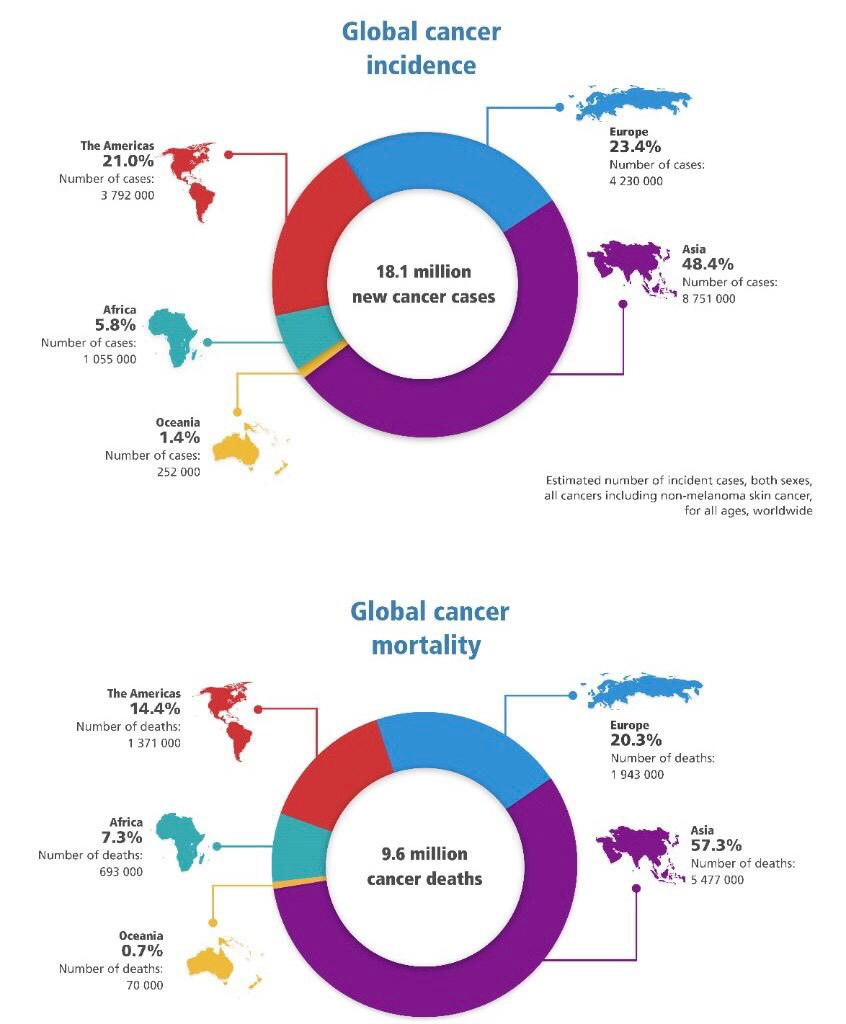
\includegraphics[width=12cm]{cancerdata}
\label{fig:cancerdata}
\end{center}
\legend{Fonte: \url{https://www.iarc.fr/wp-content/uploads/2018/09/Globocan\_01.jpg} \cite{GLOBOCAN} }
\end{figure}

\section{\textbf{Etapas do diagnóstico de câncer}}

\cite{ATLAS}.

\cite{VENCER}.

\section{\textbf{Importância do diagnóstico precoce}}

\cite{DIAGNOSTICO}.


\chapter{Inteligência Computacional e Saúde}
\label{chapter:inteligencia_computacional_e_saude}


\section{\textbf{Phyton}}
\cite{PYTHON}.


\begin{itemize}
\item Pandas  \cite{PANDAS}.
\item Scikit-learn \cite{SCIKIT}.
\end{itemize}

\section{\textbf{A base de dados}}
“Breast Cancer Wisconsin” (\url{https://www.kaggle.com/uciml/breast-cancer-wisconsin-data})\cite{BREASTCANCER}.



\chapter{Os Métodos de Análise}
\label{chapter:os_metodos_de_analise}

\section{\textbf{K Vizinhos Mais Próximos}}

Link para a figura \ref{fig:knearestneighbors}

\begin{figure}[!htb]
\begin{center}
\caption{K Vizinhos Mais Próximos}
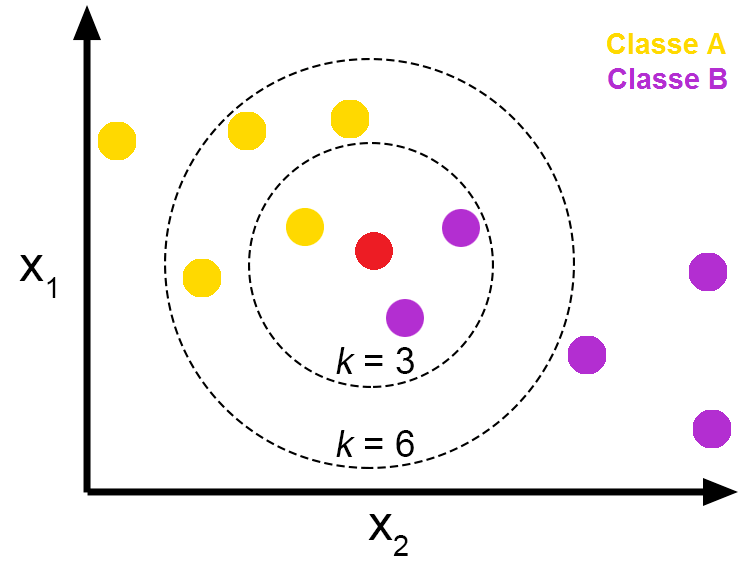
\includegraphics[width=12cm]{knearestneighbors}
\label{fig:knearestneighbors}
\end{center}
\legend{Fonte: \url{https://miro.medium.com/max/1506/0*jqxx3-dJqFjXD6FA} \cite{KNN} }
\end{figure}

\section{\textbf{Árvore de Decisão}}

Figura \ref{fig:decisiontree}

\begin{figure}[!htb]
\begin{center}
\caption{Árvore de Decisão}
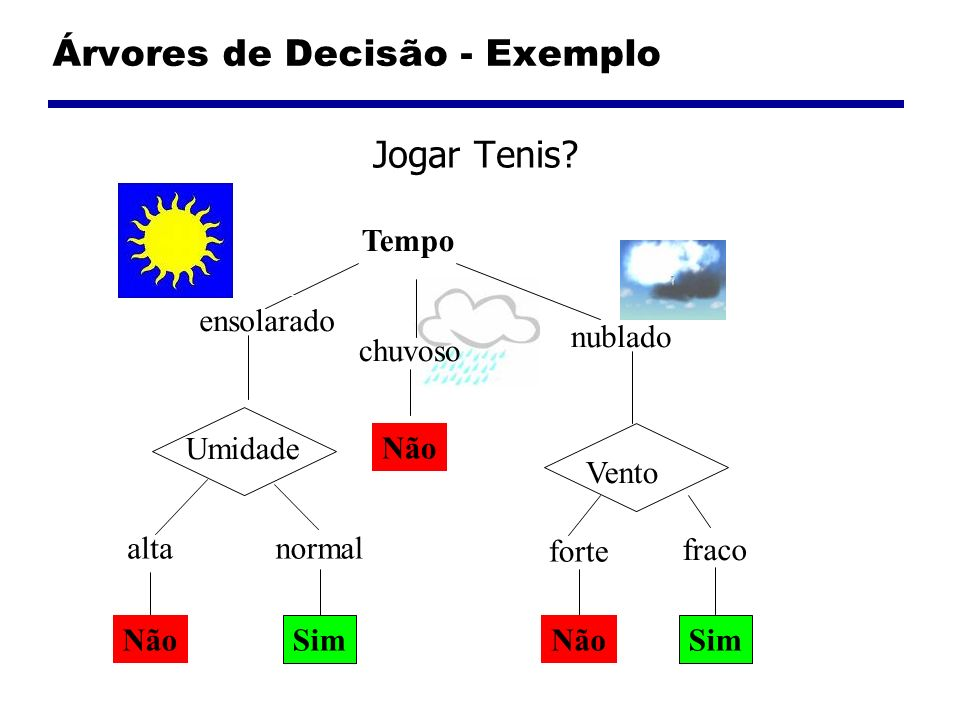
\includegraphics[width=12cm]{decisiontree}
\label{fig:decisiontree}
\end{center}
\legend{Fonte: \url{https://slideplayer.com.br/slide/358847/2/images/5/\%C3\%81rvores+de+Decis\%C3\%A3o+-+Exemplo.jpg}\cite{ARVOREDECISAO}}
\end{figure}


\section{\textbf{Floresta Aleatória}}

Figura \ref{fig:randomforest}.


\begin{figure}[!htb]
\begin{center}
\caption{Floresta Aleatória}
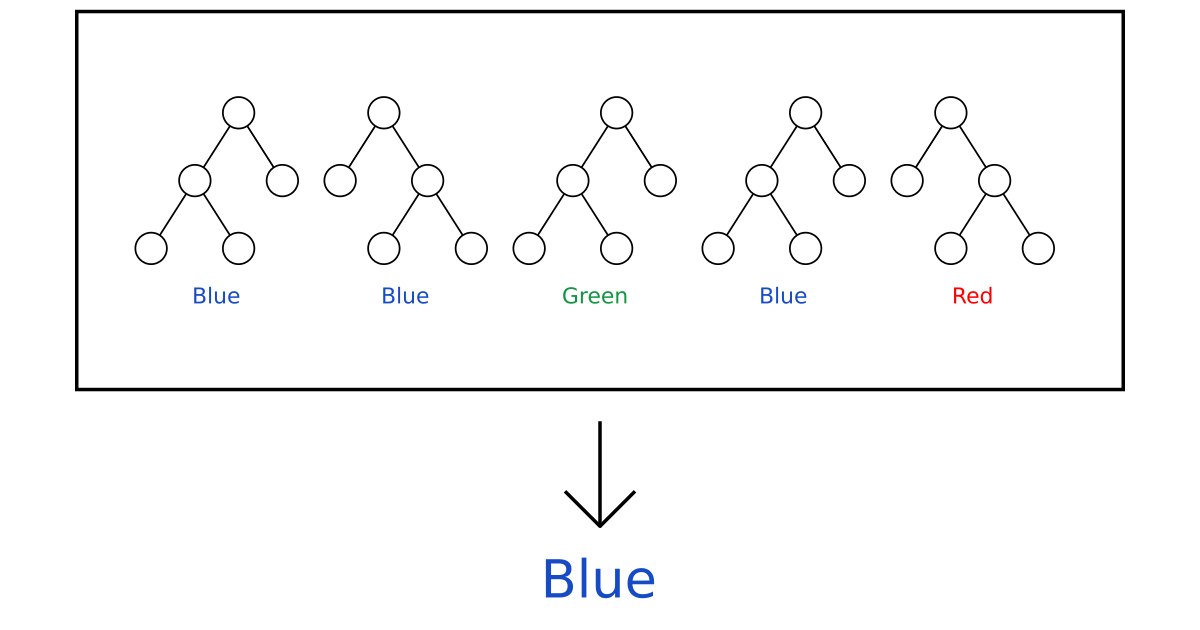
\includegraphics[width=12cm]{randomforest}
\label{fig:randomforest}
\end{center}
\legend{Fonte: \url{https://www.paradigmadigital.com/techbiz/machine-learning-dummies/} \cite{RANDOMFOREST} }
\end{figure}


\section{\textbf{Máquina de Vetor de Suporte}}

Figura \ref{fig:suportvectormachine}

\begin{figure}[!htb]
\begin{center}
\caption{Máquina de Vetor de Suporte}
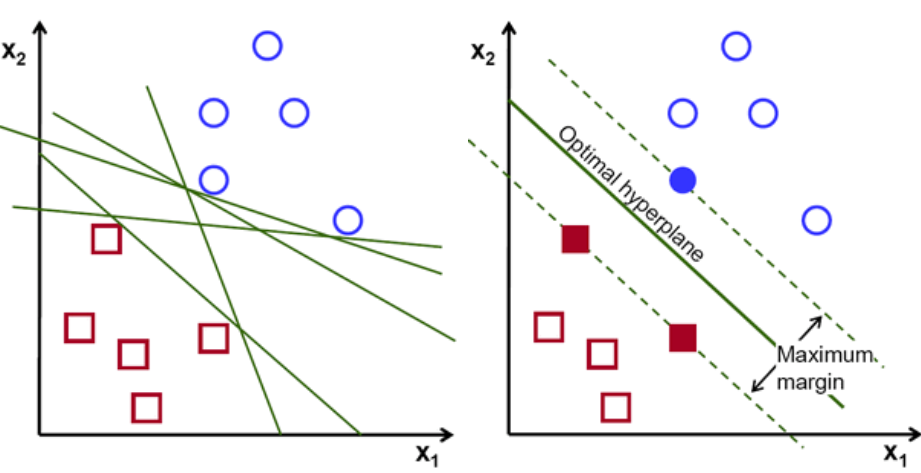
\includegraphics[width=12cm]{suportvectormachine}
\label{fig:suportvectormachine}
\end{center}
\legend{Fonte: \url{https://www.codigofluente.com.br/wp-content/uploads/2019/06/SVM04.png} \cite{SVM} }
\end{figure}

\section{\textbf{Naive bayes}}

\begin{figure}[!htb]
\begin{center}
\caption{Naive Bayes}
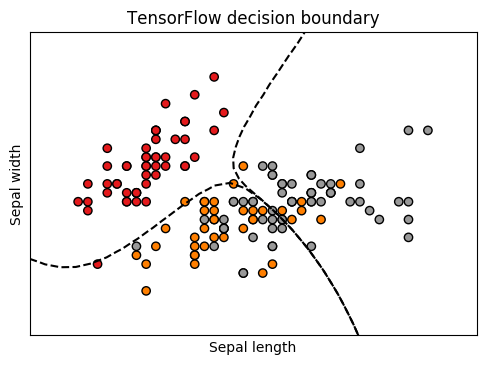
\includegraphics[width=12cm]{naivebayes}
\end{center}
\legend{Fonte: \url{https://www.researchgate.net/profile/Paolo\_Dellaversana/publication/328020065/figure/fig5/AS:677213301121033@1538471641906/Naive-Bayes-classification-of-three-different-rock-types-based-on-nine-mineralogical.png} \cite{NAIVEBAYES} }
\end{figure}

\section{\textbf{Artificial Neural Network}}


\begin{figure}[!htb]
\begin{center}
\caption{Artificial Neural Network}
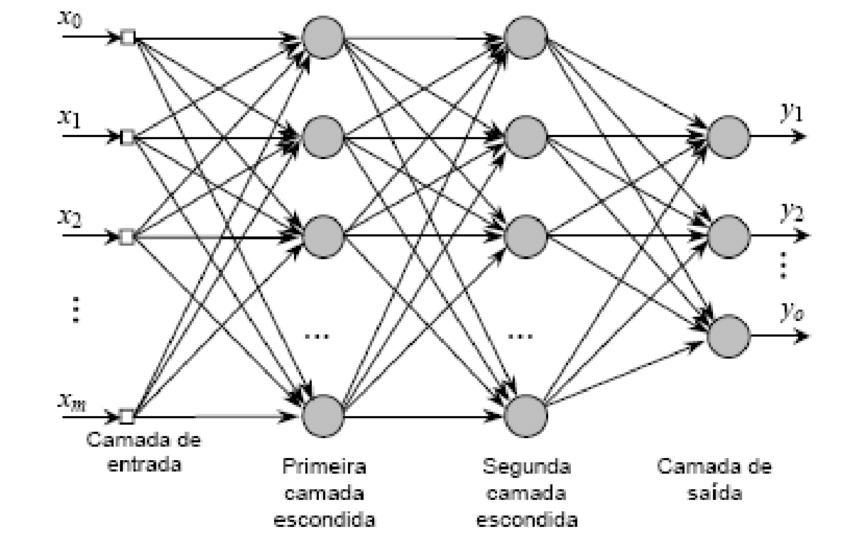
\includegraphics[width=12cm]{mlp}
\end{center}
\legend{Fonte: \url{https://www.researchgate.net/profile/Anderson\_Oliveira6/publication/240772105/figure/fig2/AS:667857415319554@1536241024122/Figura-1-Rede-Neural-Artificial-Multicamadas.png} \cite{MLP} }
\end{figure}



\chapter{O Script do Câncer de Mama}
\label{chapter:o_script_do_cancer_de_mama}


No apêndice \ref{app:code}, seção
\ref{lst:code}, página \pageref{lst:code}.
Na seção \ref{sintaxe}.

 \cite{PYTHON} 
  \ref{app:code} 
  
(\url{https://www.kaggle.com/uciml/breast-cancer-wisconsin-data/download}) \cite{BREASTCANCER}.

executa-se:

\begin{lstlisting}[language=Python, caption=Executar Script.py]
python script.py
\end{lstlisting}

\section{Validação Cruzada}

Na figura \ref{fig:crossvalidation}

\begin{figure}[H]
\begin{center}
\caption{Validação Cruzada}
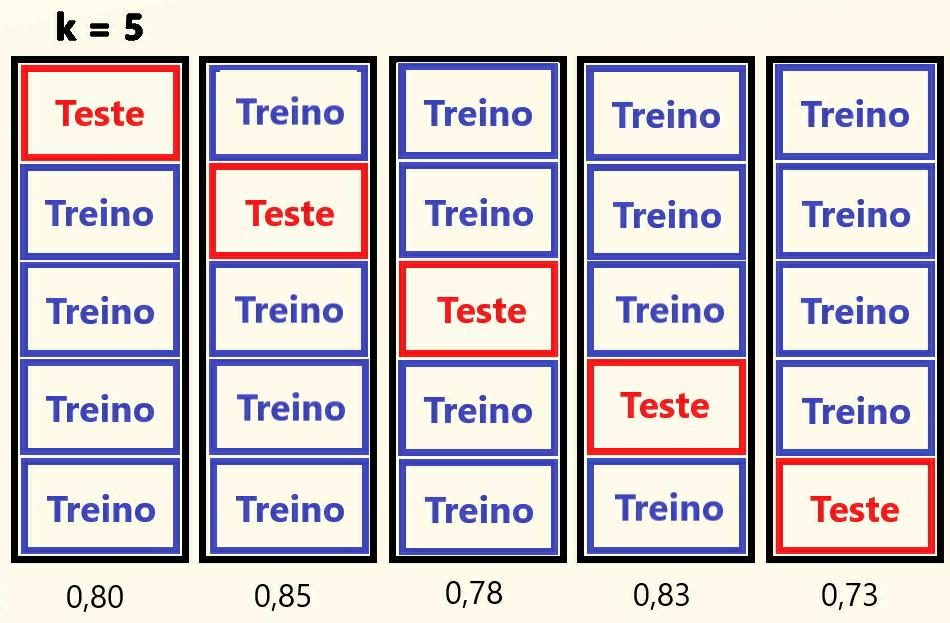
\includegraphics[width=12cm]{crossvalidation}
\label{fig:crossvalidation}
\end{center}
\legend{Fonte: \url{https://didatica.tech/wp-content/uploads/2019/10/Kfold_Resultados.png} \cite{CROSSVALIDATION} }
\end{figure}

\section{Sintaxe}
\label{sintaxe}
É chamada na primeira linha do código \ref{alg:simples}.


\begin{lstlisting}[language=Python, caption=Sintaxe Simples, label=alg:simples]
svm = SVC(kernel='poly',degree=1)
scores = cross_val_score(svm, X, y, cv=10, scoring='accuracy')
function_print = 'SuppotVectorMachine:\t' + str(scores.mean())
print(function_print)
if scores.mean() > best_score:
  best_score = scores.mean()
  best_function=function_print
\end{lstlisting}

\ref{alg:parametro},

\begin{lstlisting}[language=Python, caption=Sintaxe com Parâmetro, label=alg:parametro]
max_score = 0
for n in range(1,10):
  tree = DecisionTreeClassifier(max_depth=n, random_state=0)
  scores = cross_val_score(tree, X, y, cv=10, scoring='accuracy')
  if  scores.mean() > max_score:
    max_score = scores.mean()
    max_n = n
function_print = 'DecisionTreeClassifier:\t' + str(max_score) + '\t(max_depth=' + str(max_n) + ')'
print(function_print)
if max_score > best_score:
  best_score = max_score
  best_function=function_print
\end{lstlisting}

Tabela \ref{tab:resultado}.

\setlength{\arrayrulewidth}{0.6mm}
\begin{table}[h!]
\centering
\begin{tabular}{ |c|c|c| }
 \hline
 Função                   & Acurácia           & Parâmetro  \\
 \hline
 KneighborsClassifier     & 0.9297619047619048 & n\_neighbors = 8  \\
 DecisionTreeClassifier   & 0.9280701754385964 & max\_depth = 5    \\
 RandomForestClassifier   & 0.9649122807017543 & max\_depth = 80   \\
 SuppotVectorMachine      & 0.9051065162907269 &                   \\
 GaussianNB               & 0.9367794486215537 &                   \\
 MLPClassifier            & 0.8963032581453634 &                   \\
 \hline
 \hline
 \multicolumn{3}{|c|}{ Melhor Função} \\
 \hline
 RandomForestClassifier:  & 0.9649122807017543 & max\_depth = 80   \\
 \hline
\end{tabular}
  \caption{Resultado Final}
\label{tab:resultado}
\end{table}










\chapter{Conclusão}
\label{chapter:conclusao}

CONCLUSÃO

\pagebreak
\chapter{Trabalhos Futuros}
\label{chapter:trabalhos_futuros}

Para os desenvolvimentos de novos trabalhos na área, sugere-se, o desenvolvimento de um reprodutor gráfico para demonstrar os resultados do Script de forma mais prática, e de fácil acesso, por exemplo uma interface web. 

Em relação ao código desenvolvido nesse trabalho, um outro tipo de abordagem seria sua aplicação para outras doenças, como Hipertensão, Diabetes, que tem como base para seu diagnóstico exames que características padrões.

Em relação às linguagens de programação, a Golang \cite{GO} apresenta uma maior velocidade, ao ser confrontado com outros programas já desenvolvidos, pois possui características estruturais únicas que lhe proporcionam essa vantagem. Também poderia ser utilizado o Javascript \cite{JAVASCRIPT}, levando em consideração que ele é conhecido a nível mundial, de acordo com estatísticas pois possui características únicas como frontend web, o que em sua maioria, atrai mais o público.

Portanto, há muito o que se desenvolver no campo de Inteligência Artificial voltado à Engenharia Biomédica, auxílio ao diagnóstico de outras doenças e análise de exames.

\phantompart
\postextual
\bibliography{bibliography}
\begin{apendicesenv}
  \chapter{O Código}
  \lstinputlisting[language=Python, caption=Código Final, label=lst:code]{../code/script.py}
  \label{app:code}
\end{apendicesenv}

% \begin{anexosenv}
\chapter{Título Opcional.}
Documentos não elaborados pelo autor, utilizados de fundamentação (mapas, leis, estatutos).
\end{anexosenv}

\phantompart
\printindex
\end{document}
